\subsubsection{Student}
The student experience from start to finish is a much more fluid process than before, take for an example a student Jack who wishes to sign up to help find himself a job for his compulsory third year industrial placement.
  \paragraph{Sign Up:}
    The first thing Jack must do is sign up to CPP: Connect. He can choose the relevant departments he is a member of (in his case only Computing), enter a valid email address, password, and password confirmation.

    %TODO: Change seed to be Department of Mathematics
    \begin{figure}[H]\centering
    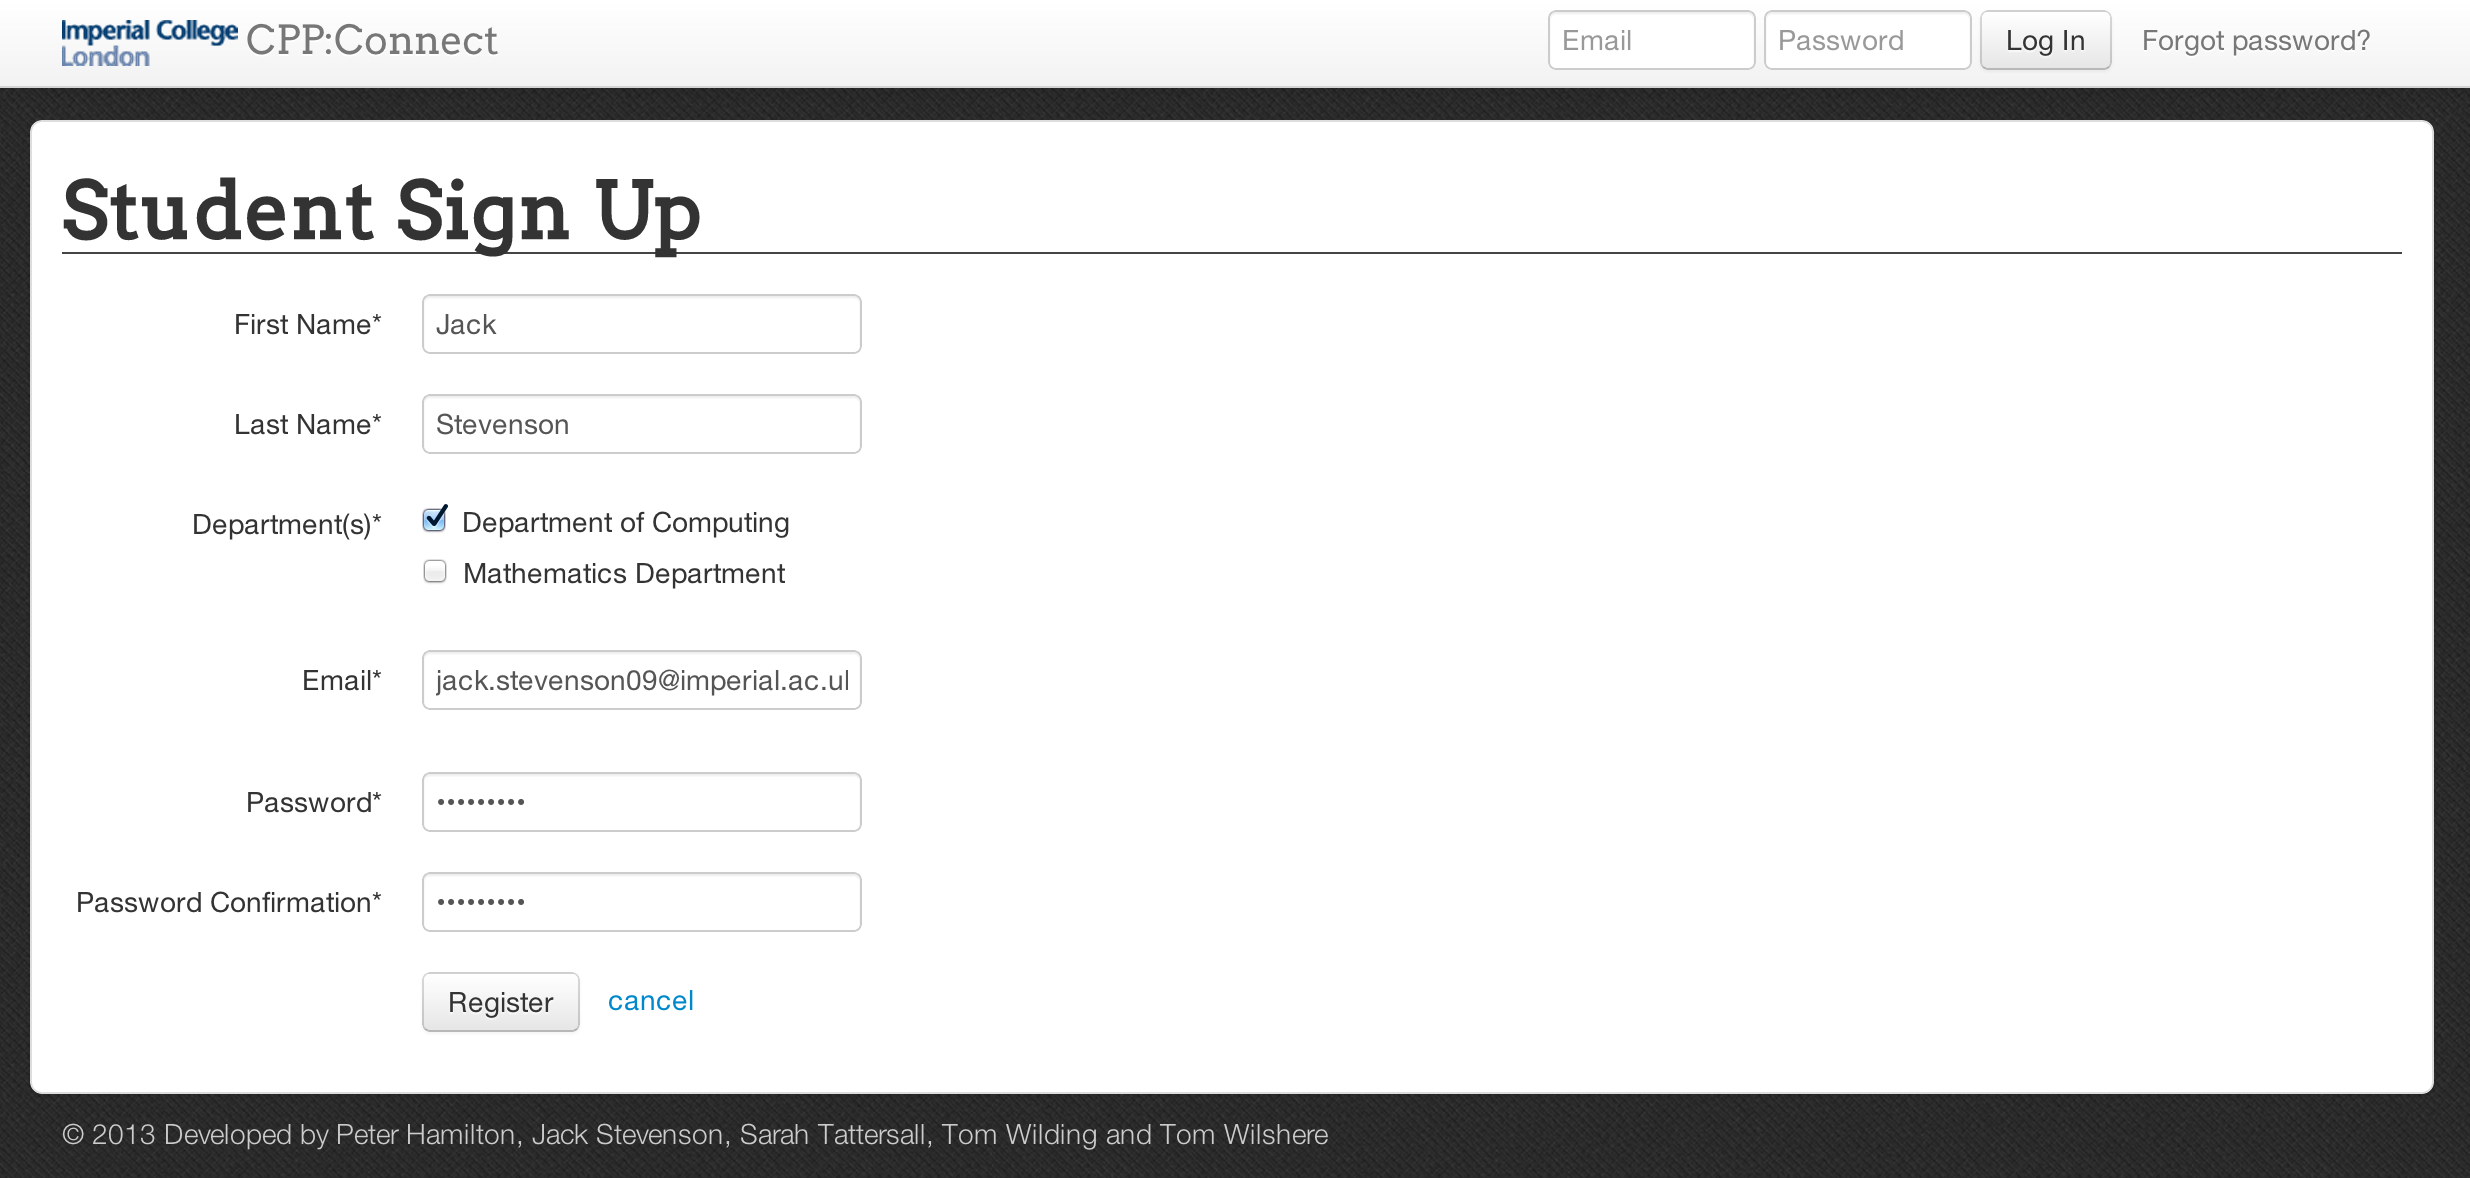
\includegraphics[scale=0.3]{images/user_experiences/student/student_signup_filled_in}
    \caption{Student sign up view}
    \end{figure}

    In order to sign up Jack must have a valid Imperial email address, if he attempts to use a different email address it will be flagged. We have used this as a technique to only allow students from a particular organisation to sign up.

    \begin{figure}[H]\centering
    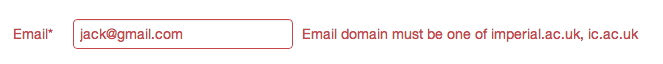
\includegraphics[scale=0.5]{images/user_experiences/student/invalid_email}
    \caption{Message displayed when student enters invalid email}
    \end{figure}

  \paragraph{Dashboard:}
    Finally when all of Jack's details are correct he proceeds to his dashboard. In order to not waste companies' time with students that have not filled in the minimal detail requirements we do not show Jack's profile just yet. In order to show up he needs at minimum a year, degree, and CV which he is made aware of via an alert box at the top of his profile whenever he visits his dashboard.

    \begin{figure}[H]\centering
    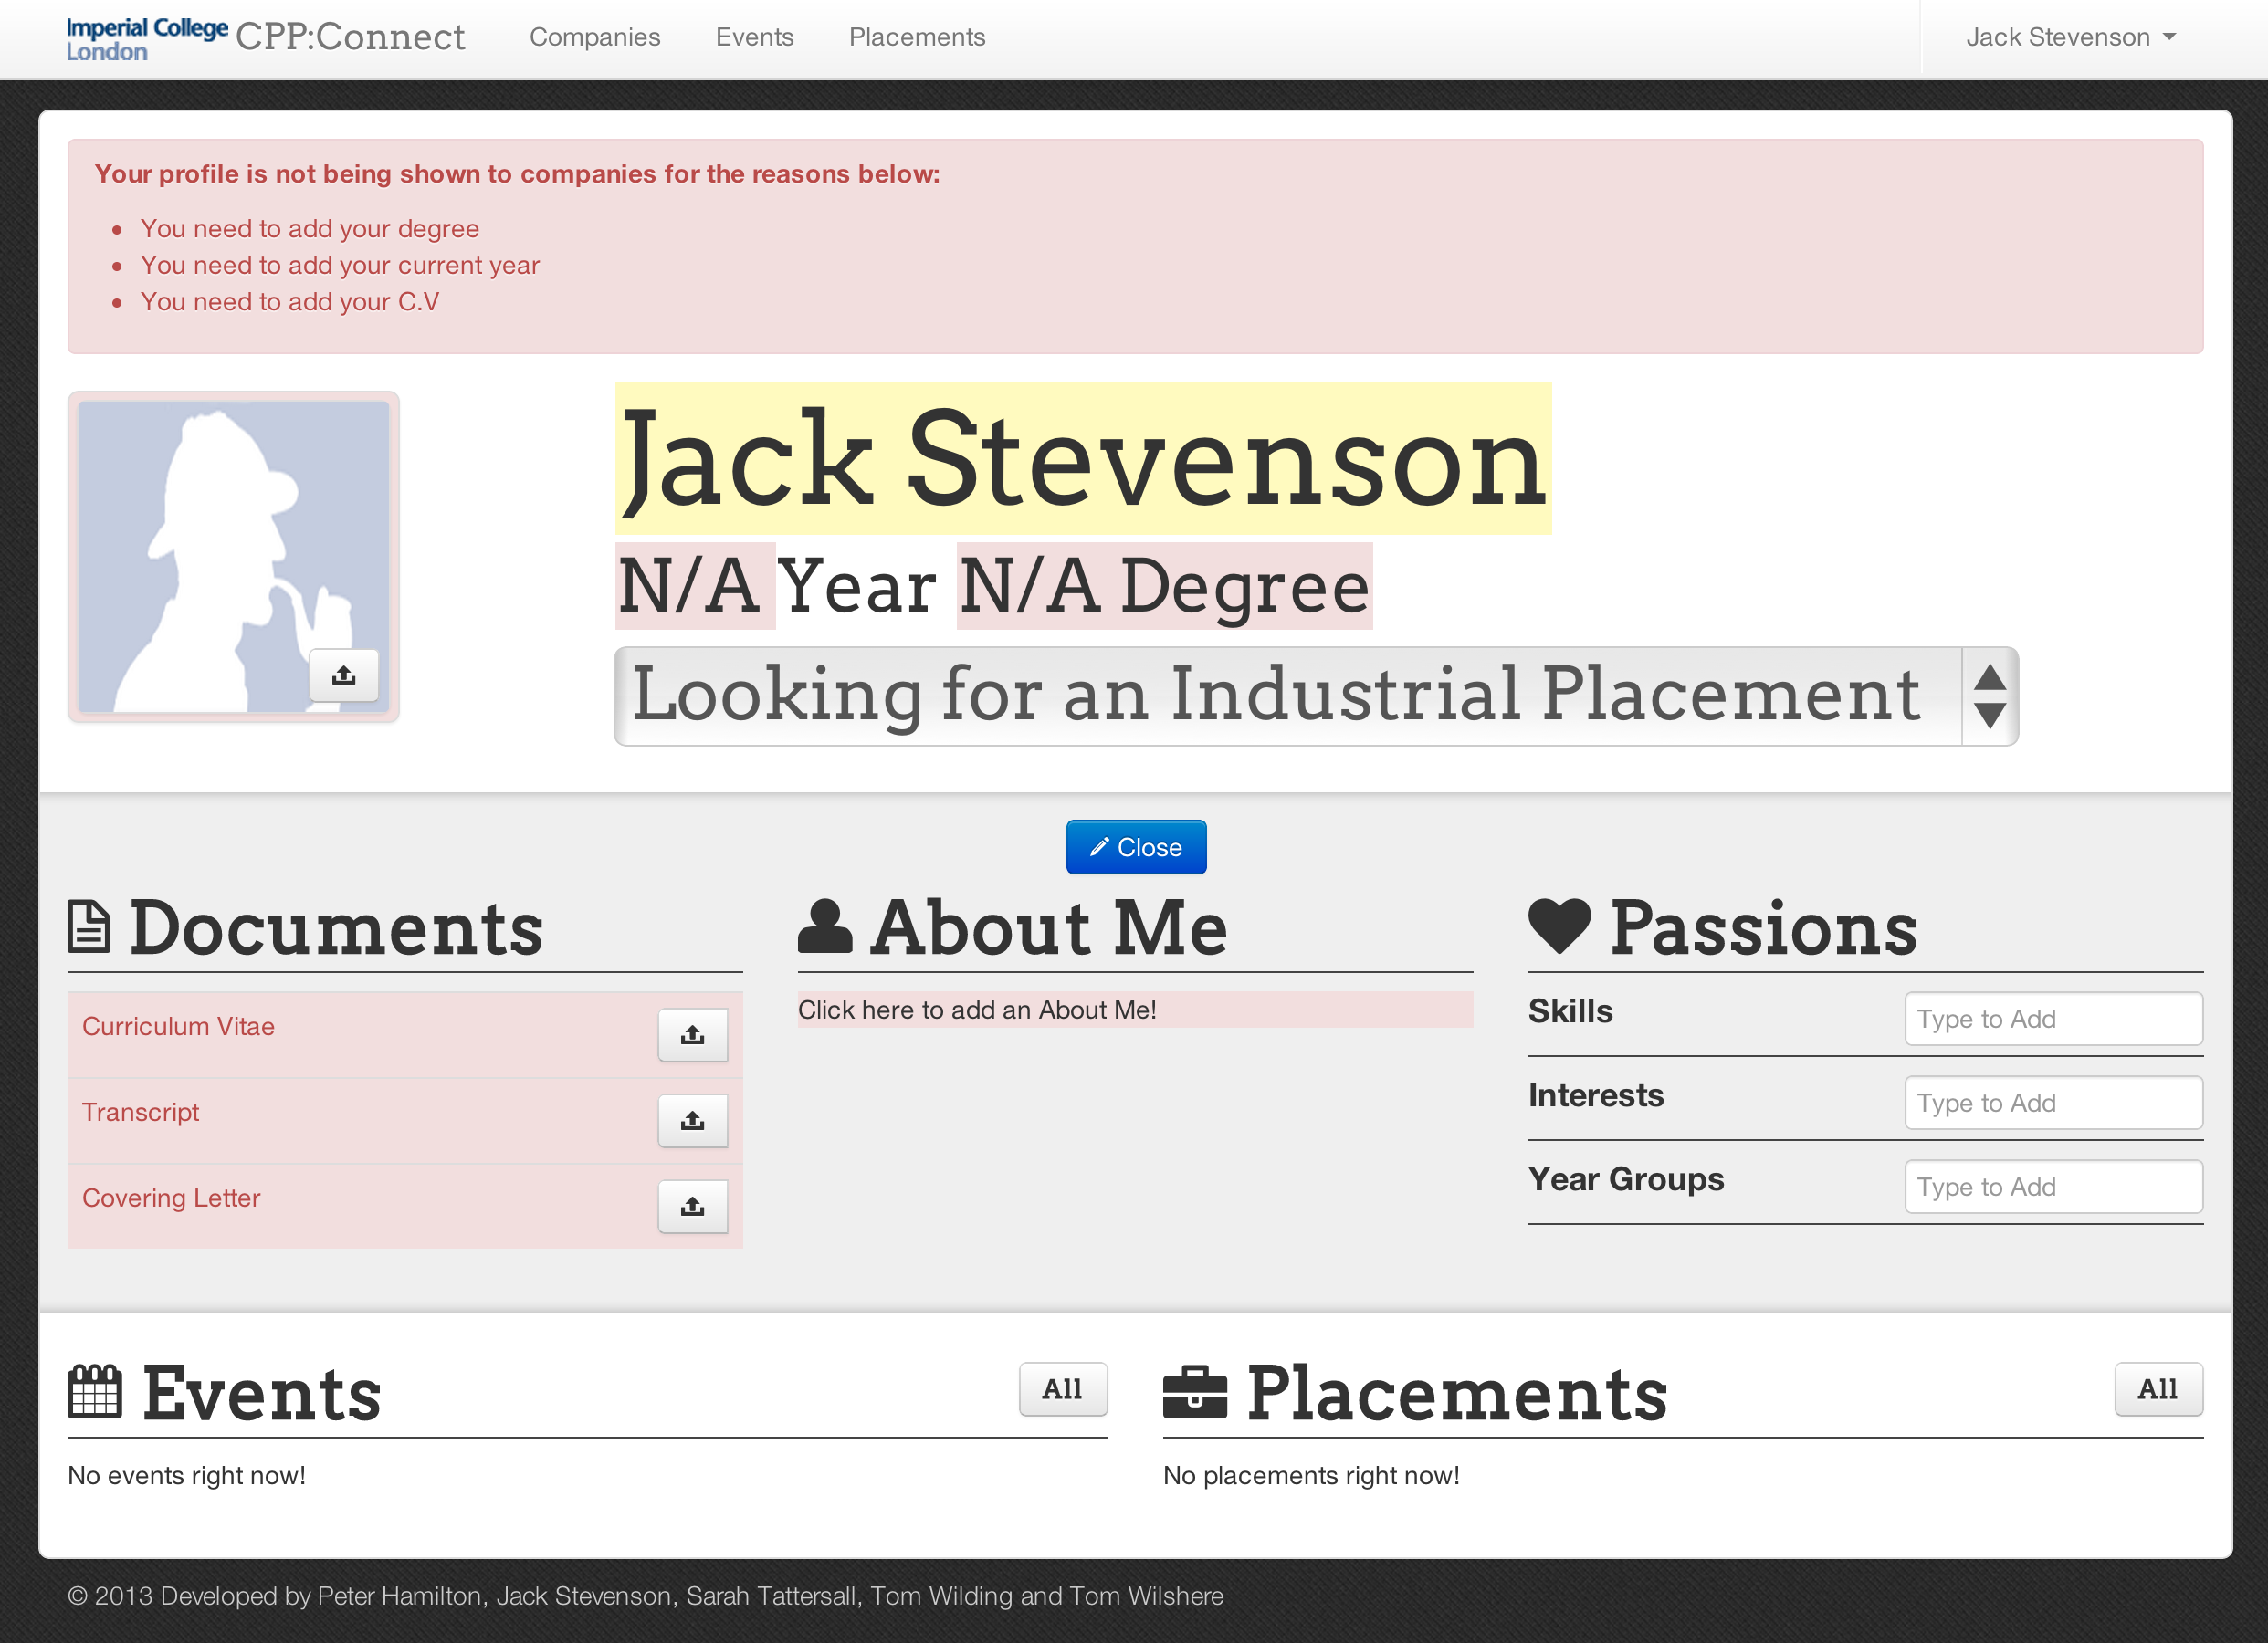
\includegraphics[scale=0.3]{images/user_experiences/student/jack_signup_profile}
    \caption{Deactivated student profile}
    \end{figure}

    Jack can then fill in his details and activate his profile ready to be found by a company.
    A complete example of which can be seen below.
    
    \begin{figure}[H]\centering
    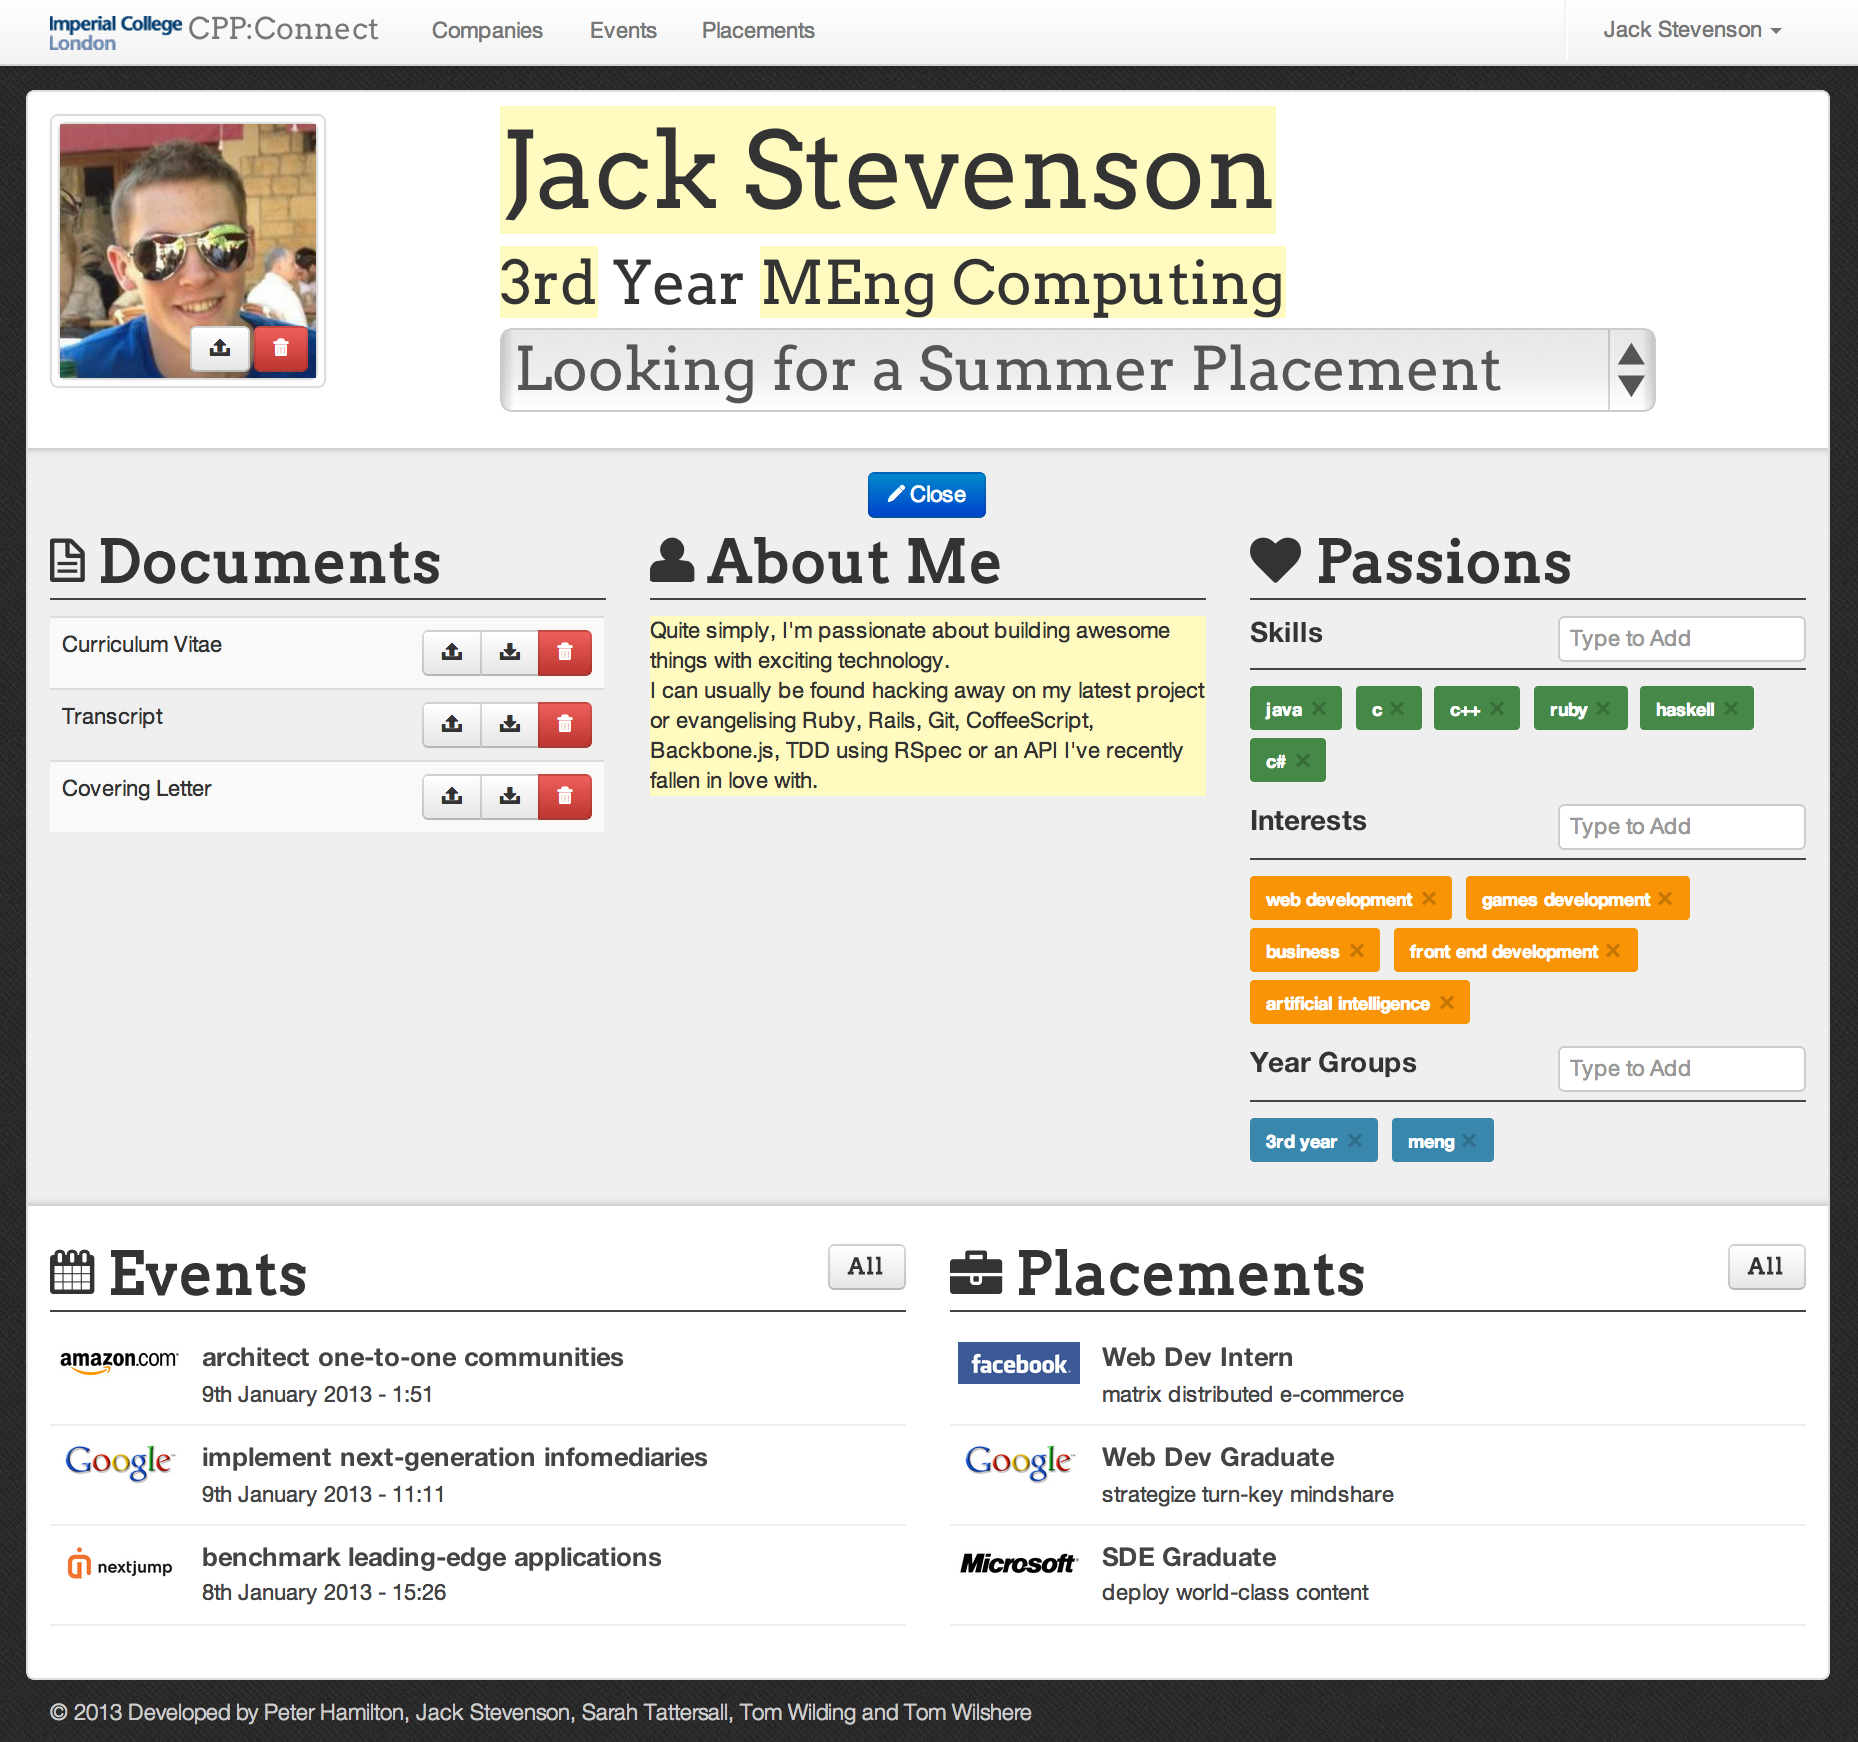
\includegraphics[scale=0.3]{images/user_experiences/student/jack_profile_complete}
    \caption{Completed student profile}
    \end{figure}

    If at any time Jack removes information which is needed in order to make his profile complete it will automatically notify him that his profile has been hidden and he must complete the information again in order to show up in any search results.

  \paragraph{Settings:}
    Jack also has an account settings page which can be accessed by clicking on his name in the navigation bar. Jack can also preview his profile as it appears to companies and log out with this too. 

    Once in his settings Jack can express if there are any skills or interests he does not wish to receive emails about when looking for a placement, toggle tool tips and whether his completed profile appears in search results, delete his profile or change his password.

    \begin{figure}[H]\centering
    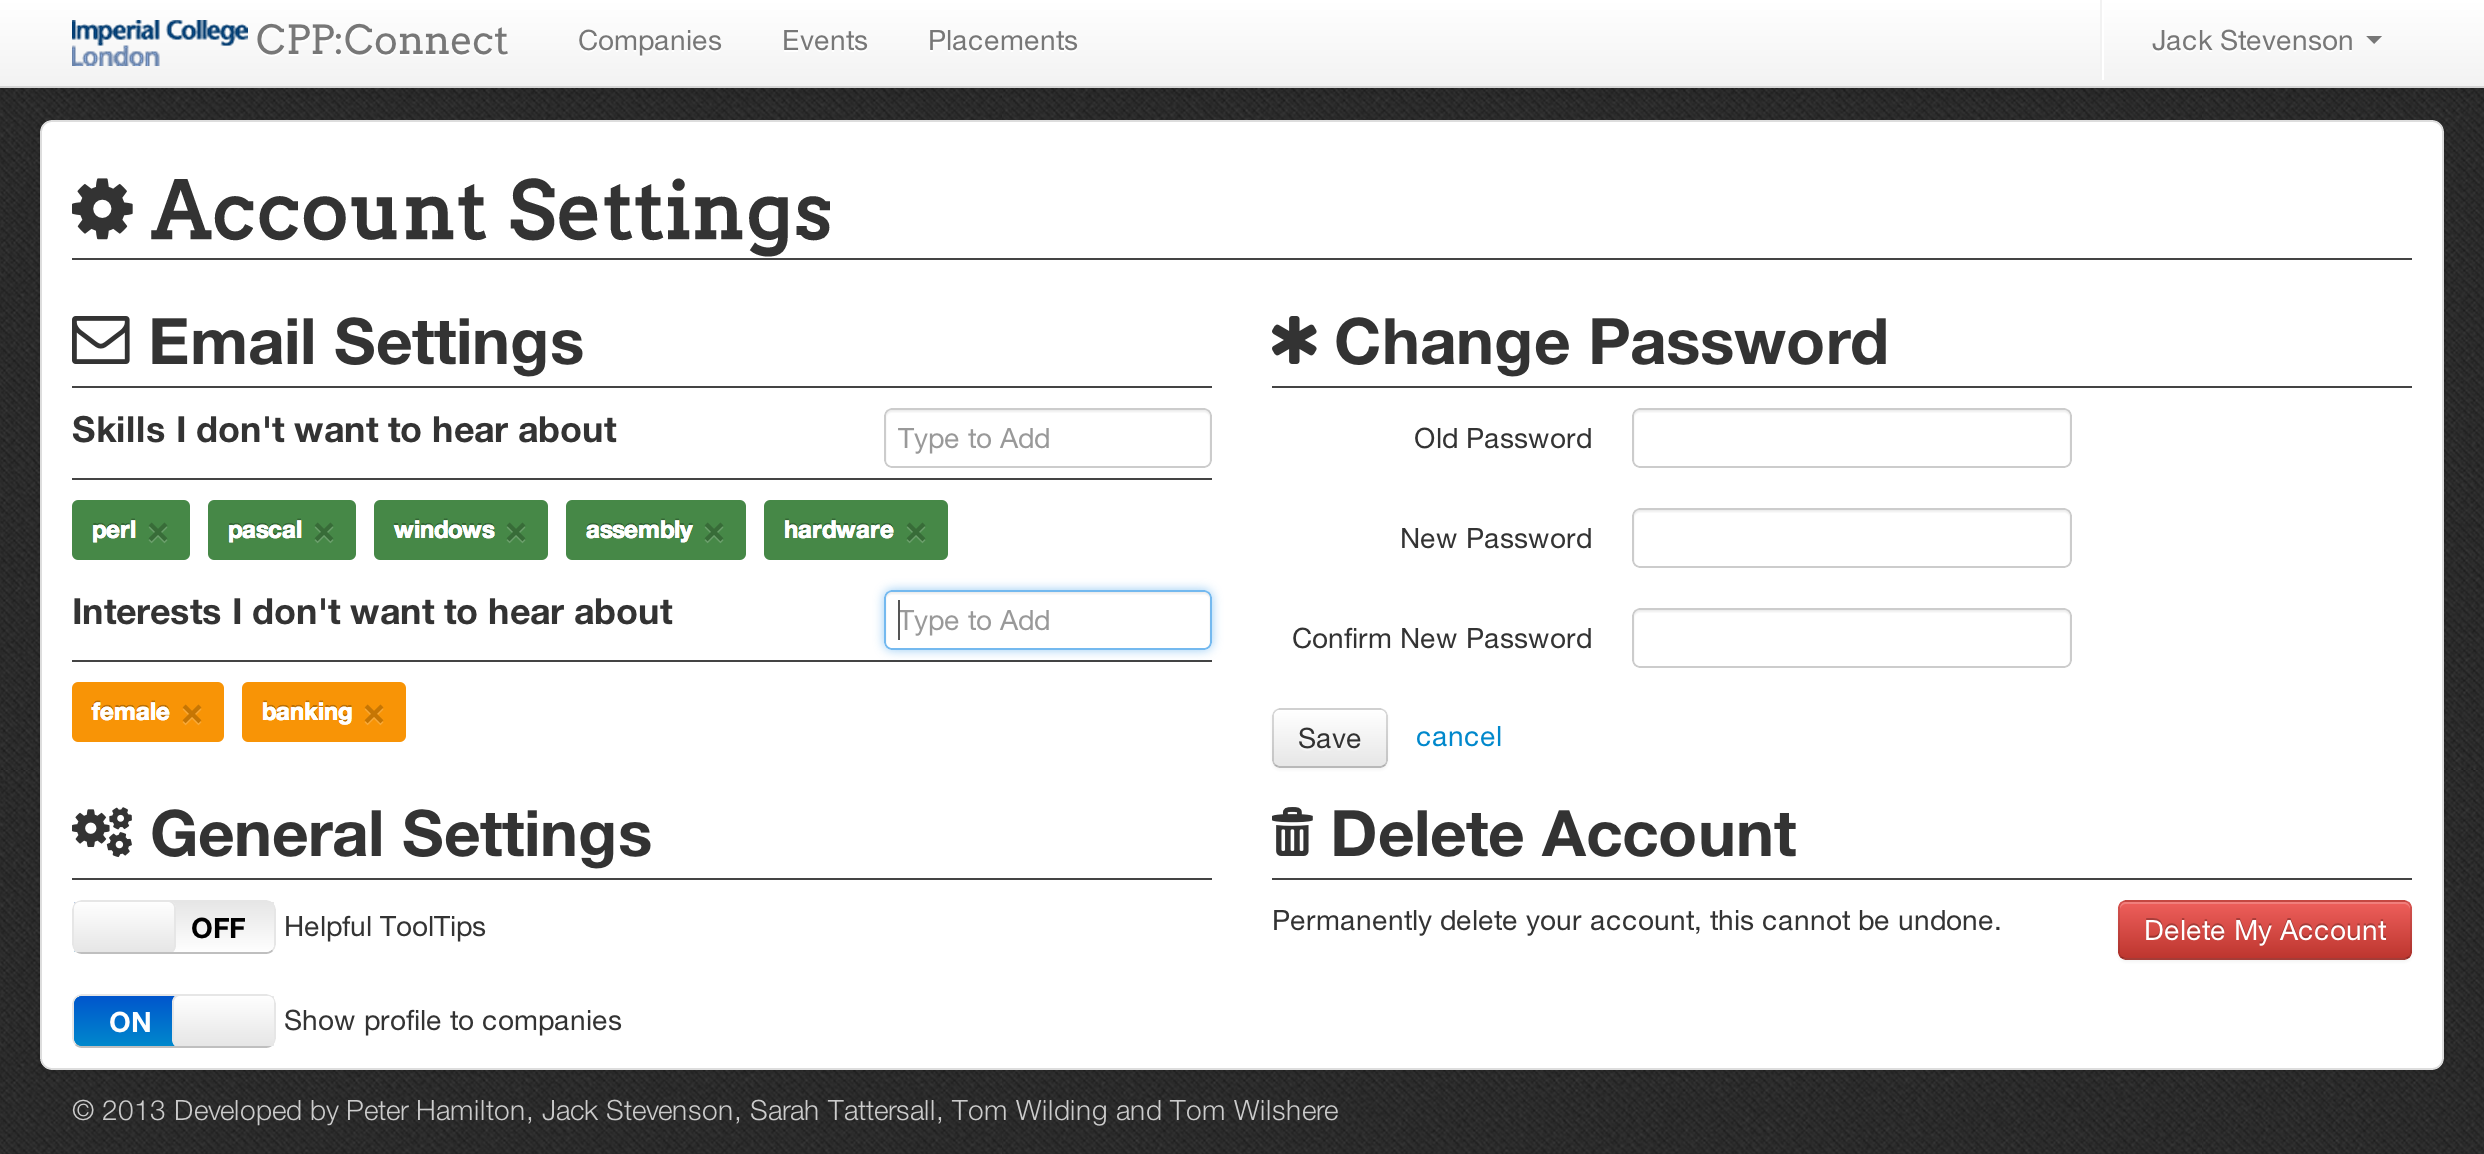
\includegraphics[scale=0.3]{images/user_experiences/student/account_settings}
    \caption{Student settings}
    \end{figure}

    Although we tell students that deleting their account is permanent, we took the design decision to actually keep old student data in the database unless purged by the administrator. This is because we may wish to view activity before they deleted themselves or in case a student accidentally deletes themselves and notifies the administrator. It is far nicer to allow them to be reinstated on the site. We found the \textit{rails3\_acts\_as\_paranoid}\cite{paranoid_gem} gem took care of this nicely for us and did not require much additional work. It will by default remove `deleted' users from any database queries so that they do not show up on our site.

  \paragraph{Events and Placements:}
    When logged in and looking at his profile, Jack can see new events and placements that have been recently advertised. By attending events students often make better personal contacts with companies than applying online and so Jack may wish to view these events by clicking on any of these or the all button to view the entire list. He can then sign up to attend events and will then receive specific email notifications about them.

    \begin{figure}[H]\centering
    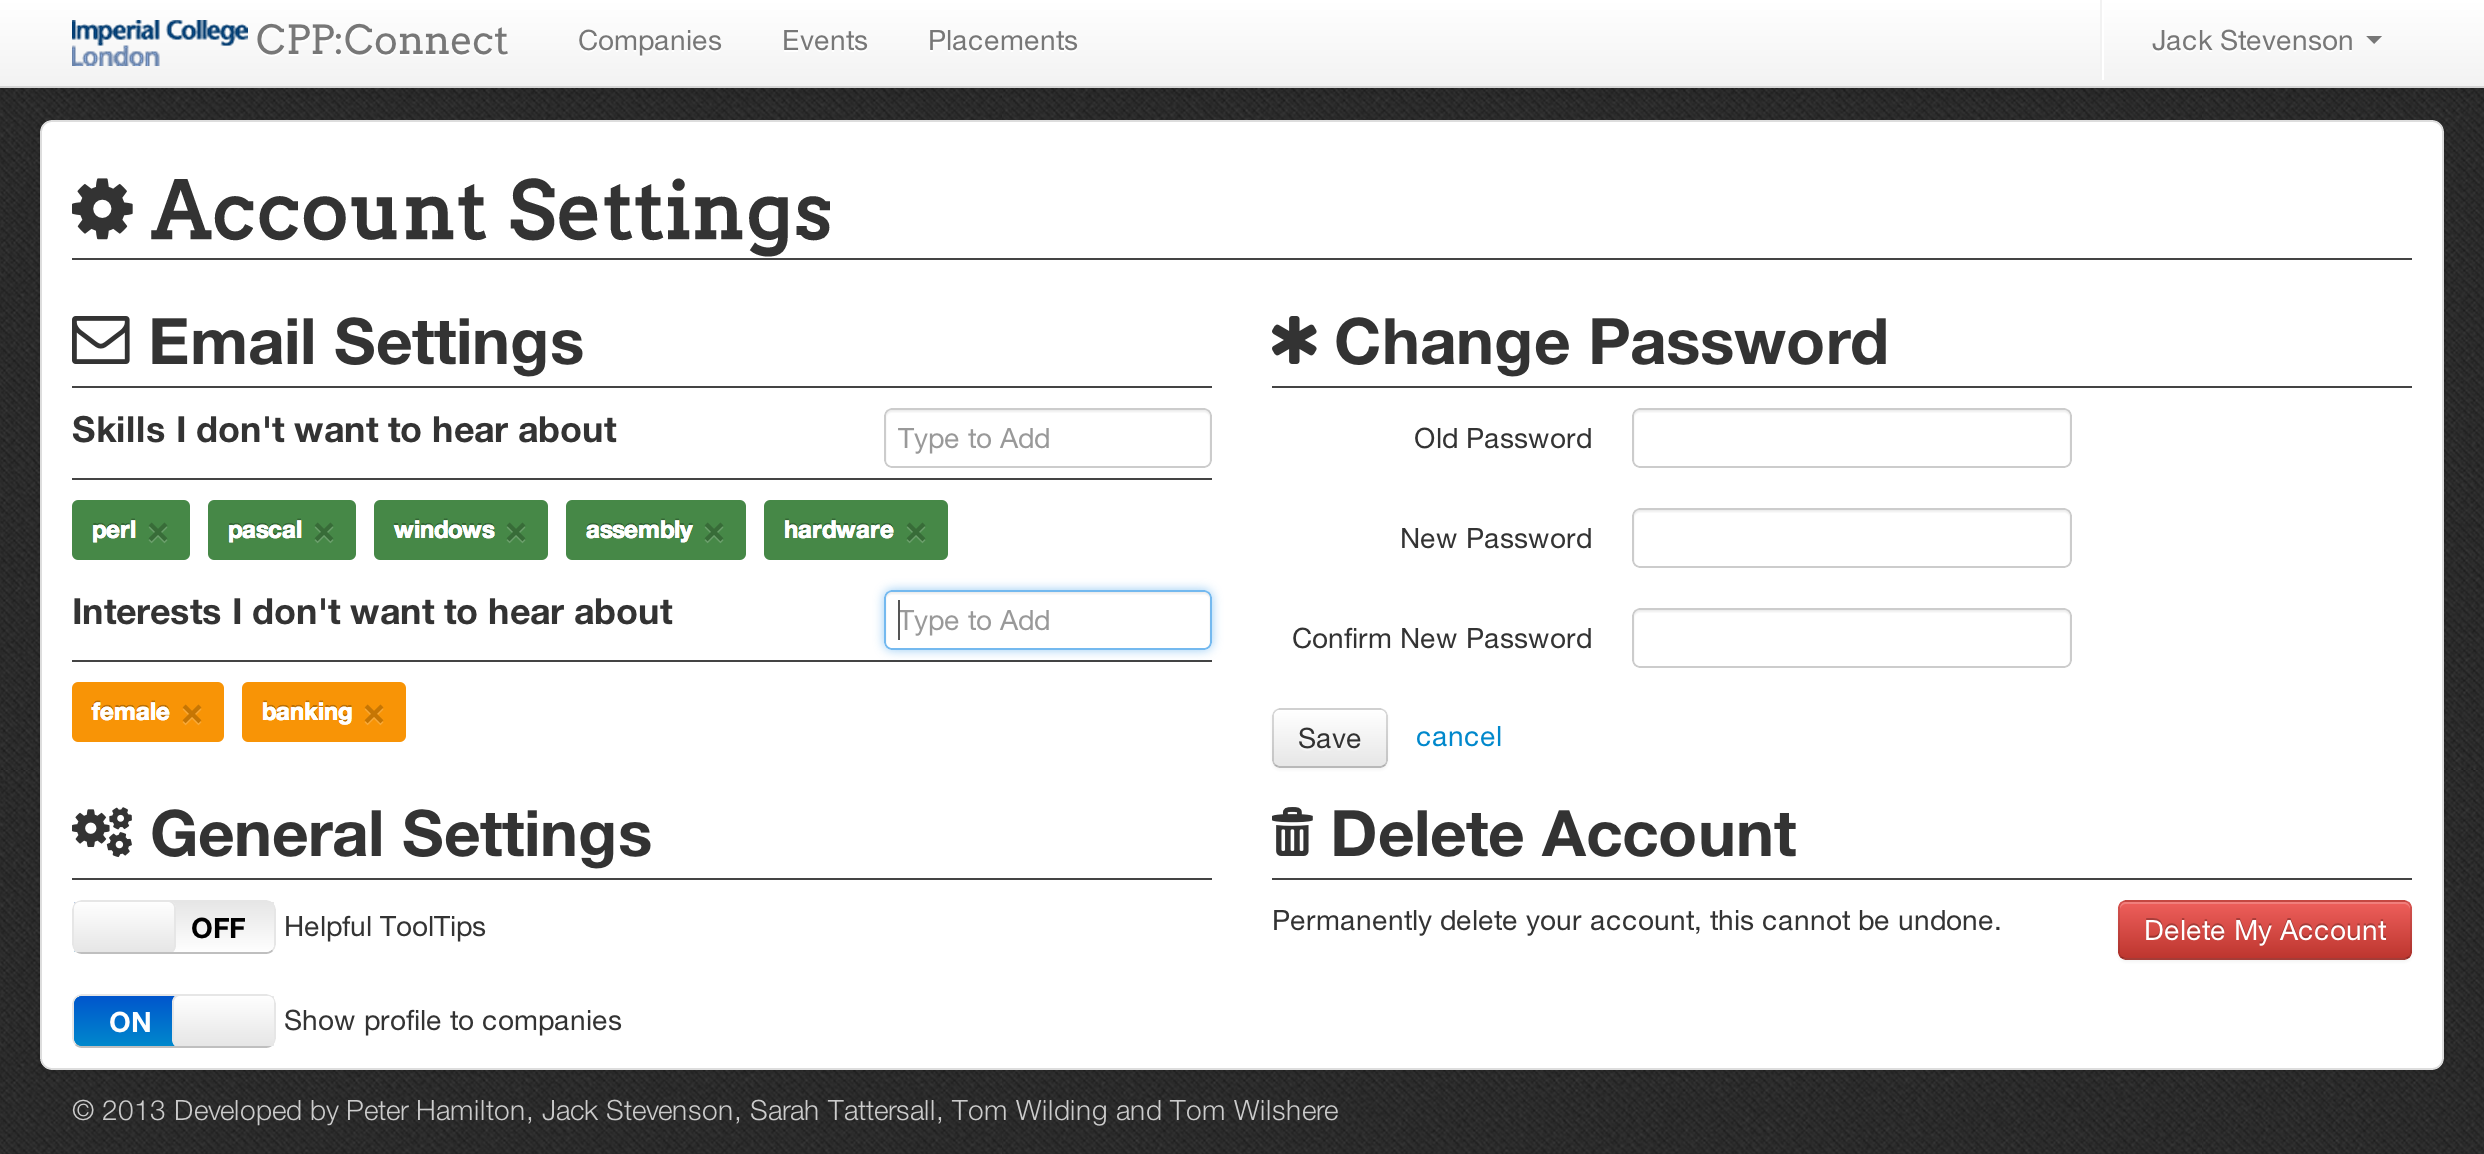
\includegraphics[scale=0.3]{images/user_experiences/student/account_settings}
    \caption{Student attending event}
    \end{figure}

    He can also browse advertised placements and send an email to any companies that advertise any he is really keen about.

  \paragraph{Companies:}
    Jack can also browse all companies, finding out a bit more about those he may not have heard of that he might be interested in working for. He does this by clicking on companies on the navigation bar and can work his way down the list, or choose to filter the list by name and/or description.
    If Jack decides he does not wish to be contacted by specific companies he can choose to blacklist them at any time. For example if Jack is not interested in a career with Netcraft and no longer wishes to receive any emails from them he can search for them on the companies list and then block them with the icon in the corner. He can also favourite companies to make sure he receives information from them, even if it contains topics he has blacklisted a tag (perhaps he might change his mind on Perl if it's at the right company?).

    Companies can also be blocked/favourited on their view page.

    %TODO: REDO PICS, REMEMBER TO USE SEARCH FEATURE
    \begin{figure}[H]\centering
    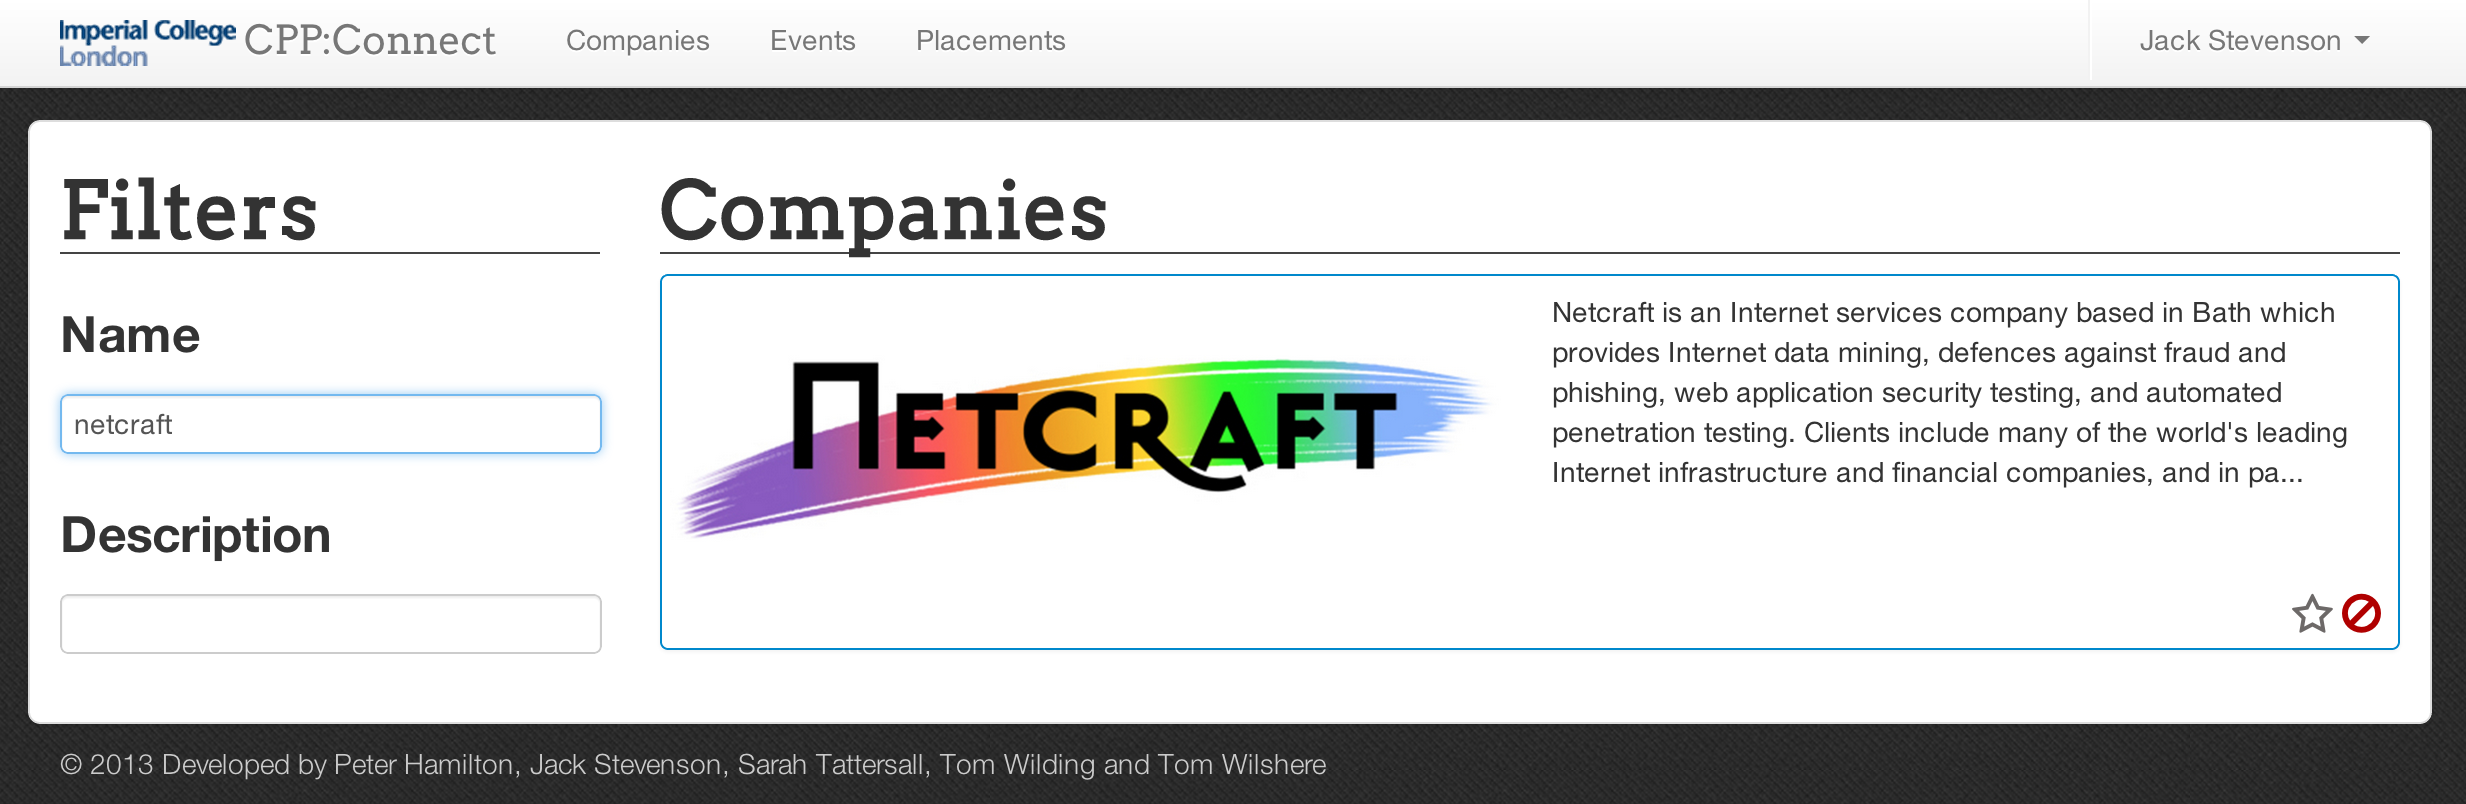
\includegraphics[scale=0.3]{images/user_experiences/student/block_netcraft}
    \caption{Students can block or favourite companies}
    \end{figure}

  \paragraph{Whilst away:}
    Once Jack has finished on the site he can log out and come back any time he wishes to use it. Companies can view his profile and he'll receive emails from any that wish to contact him.

  \paragraph{In the future:}
    If Jack should wish to deactivate his profile at a later date, he can easily do so via the deactivation option in his settings, and can re-active it in the exact same manner. Whilst deactivated Jack can still view and sign up to events as well as view placements and companies. He may choose to deactivate it in order to not appear in any company searches because his information is not up to date and will require some time to fix, or he might have obtained a placement and does not wish to advertise himself any longer.

    Should Jack ever forget his password he can always click on the `forgot password?' link provided in the navigation bar when he reaches the landing page. This will take him to a form where he enters his email address. Once submitted, Jack's password is reset to a secure random eight character string which is automatically generated and then emailed to him. He is also advised in the email to change his new password straight away, which can be done via the settings page as described above.